\documentclass[a4paper,10pt]{article}
\usepackage[utf8]{inputenc}
\usepackage[T1]{fontenc}
\usepackage{amsmath, amssymb, amsthm}
\usepackage{pgfplots}
\pgfplotsset{compat=1.16}

\begin{document}

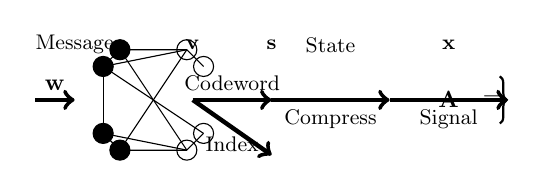
\begin{tikzpicture}[every node/.style={scale=0.85}]
	\tikzset{LDPC/.pic={
		\draw[pic actions] (-0.75,-0.5)--(-0.75,0.5);
		\draw[pic actions] (-0.5,0.75)--(0.5,0.75)--(0.75,0.5);
		\draw[pic actions] (-0.5,-0.75)--(0.5,-0.75)--(0.75,-0.5);
		\draw[pic actions] (-0.75,0.5)--(0.75,-0.5);
		\draw[pic actions] (-0.5,0.75)--(0.5,-0.75);
		\draw[pic actions] (-0.5,-0.75)--(0.5,0.75);
		\draw[pic actions] (-0.5,0.75)--(0.5,0.75);
		\draw[pic actions] (-0.5,-0.75)--(0.5,-0.75);
		\draw[pic actions] (-0.75,0.5)--(-0.5,0.75);
		\draw[pic actions] (-0.75,-0.5)--(-0.5,-0.75);
		\draw[pic actions] (-0.75,0.5)--(0.5,0.75);
		\draw[pic actions] (-0.75,-0.5)--(0.5,-0.75);
		\filldraw[pic actions] (-0.75,0.5) circle (0.15);
		\filldraw[pic actions] (-0.5,0.75) circle (0.15);
		\filldraw[pic actions] (-0.75,-0.5) circle (0.15);
		\filldraw[pic actions] (-0.5,-0.75) circle (0.15);
		\draw[pic actions] (0.5,0.75) circle (0.15);
		\draw[pic actions] (0.75,0.5) circle (0.15);
		\draw[pic actions] (0.5,-0.75) circle (0.15);
		\draw[pic actions] (0.75,-0.5) circle (0.15);	
	}}
	\path (-2,0) edge[->, ultra thick] node[above] {${\mathbf{w}}$} (-1.5,0);
	\node at (-1.5,0.7) {\small Message};
	\pic at (-0.5,0) {LDPC};
	\path (0,0) edge[->, ultra thick] node[above] {\small Codeword} (1,0);
	\path (0,0) edge[->, ultra thick] node[below] {\small Index} (1,-0.7);
	\node at (0,0.7) {\small ${\mathbf{v}}$};
	\node at (1,0.7) {\small ${\mathbf{s}}$};
	\path (1,0) edge[->, ultra thick] node[below] {\small Compress} (2.5,0);
	\node at (1.75,0.7) {\small State};
	\path (2.5,0) edge[->, ultra thick] node[below] {\small Signal} (4,0);
	\node at (3.25,0.7) {\small ${\mathbf{x}}$};
	\node at (3.25,0) {$\mathbf{A}$};
	\node at (3.8,0) {$=$};
	\draw [decorate,decoration={brace,raise=1mm},thick] (3.8,0.3) -- (3.8,-0.3);
	\end{tikzpicture}

\end{document}